\section{Optimierung der Empfehlungsqualität}
% V-Ansatz Teil 3 – Evaluation und Optimierung
\subsection{Zielfunktion}
\label{sec:target_function}
Als Zielfunktion für die Optimierung des hybriden Empfehlungssystems dient eine gewichtete 
Linearkombination der Scores der beiden zugrundeliegenden Modelle. Dieser Ansatz wurde 
aufgrund seiner einfachen Interpretierbarkeit und seiner weiten Verbreitung als robuste 
Baseline für hybride Architekturen gewählt (vgl. \cite{burke_hybrid_2002}). 
Die mathematische Formulierung der Funktion lautet:

\begin{equation}
\label{eq:target}
s_\mathrm{hybrid} = w_\mathrm{cbf} \cdot s_\mathrm{cbf} + w_\mathrm{cf} \cdot s_\mathrm{cf}
\end{equation}

Die einzelnen Terme der Gleichung sind wie folgt definiert:
\begin{itemize}
    \item $s_\mathrm{hybrid}$: Der finale, kombinierte Score für ein potenziell zu empfehlendes Item. 
    Die finale Empfehlungsliste wird durch das absteigende Sortieren der Items nach diesem Score erstellt.
    
    \item $s_\mathrm{cbf}$ und $s_\mathrm{cf}$: Die von der Content-Based- bzw. der Collaborative-Filtering-Komponente 
    generierten Roh-Scores. Vor der Kombination in der Zielfunktion ist eine Normalisierung dieser 
    Scores erforderlich, um sicherzustellen, dass sie auf einer vergleichbaren Skala liegen.
    
    \item $w_\mathrm{cbf}$ und $w_\mathrm{cf}$: Die nicht-negativen Gewichtungsparameter, welche den Einfluss 
    der jeweiligen Modellkomponente auf das Endergebnis steuern. Für diese Gewichte gilt die Nebenbedingung 
    $w_\mathrm{cbf} + w_\mathrm{cf} = 1$, wodurch die Optimierung auf die Bestimmung eines einzigen 
    Parameters reduziert wird.
\end{itemize}

Das zentrale Ziel des in~\ref{sec:opt_strat} beschriebenen Optimierungsprozesses 
ist es, die optimalen Werte für die Gewichtungsparameter $w_\mathrm{cbf}$ und $w_\mathrm{cf}$ zu finden, 
sodass die in Abschnitt~\ref{sec:metrics} definierte Evaluationsmetrik (nDCG@10) maximiert wird.

\subsection{Evaluationsmetriken}
\label{sec:metrics}
Die empirische Bewertung und Optimierung des hybriden Empfehlungssystems erfordert ein klar definiertes 
Evaluationsprotokoll sowie eine geeignete Zielfunktion. Als primäre Zielfunktion für die in Kapitel 4 
beschriebene Hyperparameter-Optimierung dient die Maximierung der Empfehlungsqualität, gemessen durch 
den normalisierten diskontierten kumulativen Gewinn bei einer Listenlänge von 10 (nDCG@10). Diese Metrik 
wurde ausgewählt, da sie nicht nur die reine Trefferquote erfasst, sondern vor allem die exakte Position 
eines relevanten Treffers innerhalb der Empfehlungsliste gewichtet, was das reale Nutzerverhalten präzise abbildet.

Die besondere Eignung des nDCG als Metrik für Empfehlungssysteme liegt in seiner positions-sensitiven 
("top-heavy") Natur. Mathematisch wird dies durch eine logarithmische Diskontierung erreicht, bei der der 
Wert eines Treffers am Rang $r$ mit dem Faktor $1/\log_2(r+1)$ abgewertet wird. Dies führt dazu, dass ein 
Treffer an den vordersten Rängen überproportional mehr zur Gesamtbewertung beiträgt als ein Treffer an einer 
späteren Position. So ist beispielsweise ein relevanter Artikel an Rang 1 signifikant wertvoller als 
an Rang 2, während der Unterschied zwischen Rang 100 und 101 nur noch marginal ist. Diese Eigenschaft ist 
essenziell, da Nutzer Interaktionen auf den vordersten Plätzen der Ergebnisliste konzentrieren und weiter 
hinten platzierte Vorschläge selten beachten (vgl. \cite{krichene_sampled_2020}).

Ein entscheidender Aspekt des Evaluationsdesigns ist die Handhabung negativer Instanzen. Anstatt auf 
Verfahren des Negative Samplings zurückzugreifen, bei denen eine kleine, zufällige Teilmenge 
nicht-interagierter Artikel als negative Beispiele dient, wird in dieser Arbeit eine 
methodisch rigorosere Strategie des \textit{Full-Catalog Rankings} verfolgt. Bei diesem Vorgehen muss 
das Modell für jeden positiven Testfall den relevanten Artikel aus der Gesamtheit aller im 
Datensatz verfügbaren Artikel – abzüglich der bereits vom Nutzer gelesenen – identifizieren.

Diese Methode vermeidet systematische Verzerrungen (sampling bias), die durch ein 
unausgewogenes Sampling entstehen können, und simuliert ein anspruchsvolles, aber realistisches 
Anwendungsszenario. Die Evaluation auf dem gesamten Artikelkatalog stellt eine enorme 
Herausforderung für das Empfehlungssystem dar, was naturgemäß zu absolut gesehen niedrigen 
Metrikwerten führt. Wie in der Fachliteratur bestätigt wird, sind solche Ergebnisse jedoch nicht 
als Indikator für eine geringe Modellleistung zu interpretieren, sondern als Konsequenz eines 
besonders anspruchsvollen und unverzerrten Evaluationsprotokolls 
(vgl. \cite{krichene_sampled_2020}). Die auf diese Weise gewonnenen Erkenntnisse bieten eine 
robuste und verlässliche Grundlage für die zukünftige Weiterentwicklung von 
Empfehlungssystemen bei der SV-Gruppe.

\subsection{Experimenteller Aufbau und Validierungsdatensatz}
Die Grundlage für die Optimierung und Evaluation bildet ein Validierungsdatensatz, der aus den 
Nutzerinteraktionen der letzten Januarwoche 2025 extrahiert wurde. Die statistischen Kennzahlen 
dieses Zeitraums sind in Tabelle~\ref{tab:statistiken_test} zusammengefasst.

\begin{table}[H]
    \centering
    \caption{Statistische Kennzahlen des Test- und Validierungsdatensatzes, basierend auf den Klick-Logs der letzten Januarwoche.}
    \label{tab:statistiken_test}
    \begin{tabular}{lr}
        \toprule
        \textbf{Metrik} & \textbf{Wert} \\
        \midrule
        Gesamte Interaktionen (Klicks) & 3.627.024 \\
        Einzigartige Nutzer & 1.099.289 \\
        Einzigartige Artikel & 57.100 \\
        \bottomrule
    \end{tabular}
\end{table}

Aus dem Gesamt-Pool an Nutzern wurde eine repräsentative Validierungsstichprobe von 1.000 
einzigartigen Nutzern zufällig gezogen, um den für die Optimierung erforderlichen Rechenaufwand in einem praktikablen 
Rahmen zu halten. Für jeden Nutzer in der Stichprobe wurde nach dem \textit{Leave-Last-Out}-Prinzip 
der letzte interagierte Artikel als Ground Truth für die Evaluation definiert.

\subsection{Optimierungsstrategie}
\label{sec:opt_strat}
Die Bestimmung der optimalen Gewichtungsparameter $w_\mathrm{cbf}$ und $w_\mathrm{cf}$ aus 
Gleichung~\ref{eq:target} erfolgt durch einen automatisierten Hyperparameter-Optimierungsprozess.

Als Framework für diesen Prozess wurde \textit{Optuna} gewählt, das eine effiziente Suche im 
Parameterraum ermöglicht. Über insgesamt 515 Iterationen (Trials) wurden verschiedene 
Gewichtungskombinationen evaluiert, mit dem Ziel, die in Abschnitt~\ref{sec:metrics} definierte 
nDCG@10-Metrik zu maximieren.

Der Ablauf eines einzelnen Optimierungs-Trials gestaltet sich wie folgt:
\begin{enumerate}
    \item Optuna schlägt eine neue Wertekombination für $w_\mathrm{cbf}$ und $w_\mathrm{cf}$ vor.
    \item Für jeden der 1.000 Nutzer in der Validierungsstichprobe werden die Empfehlungen der 
    \ac{CBF}- und \ac{CF}-Modelle über deren jeweilige API-Endpunkte parallel und asynchron abgerufen.
    \item Die Ergebnislisten der beiden Modelle werden mittels der vorgeschlagenen Gewichte zu einer 
    finalen hybriden Empfehlungsliste fusioniert.
    \item Der nDCG@10-Wert dieser finalen Liste wird berechnet, indem sie mit dem Ground-Truth-Artikel 
    des Nutzers verglichen wird.
    \item Der über alle 1.000 Nutzer gemittelte nDCG@10-Wert wird an Optuna zurückgegeben, um 
    den nächsten, informierteren Suchschritt zu steuern.
\end{enumerate}

Dieser Prozess entspricht einem Gesamtaufwand von 515.000 individuellen Evaluierungen des 
Hybridmodells, was eine gründliche und robuste Suche nach der optimalen Parameterkonfiguration 
gewährleistet.
% content/figures/plot_hyperparameterraum.tex

\begin{figure}[H]
    \centering
    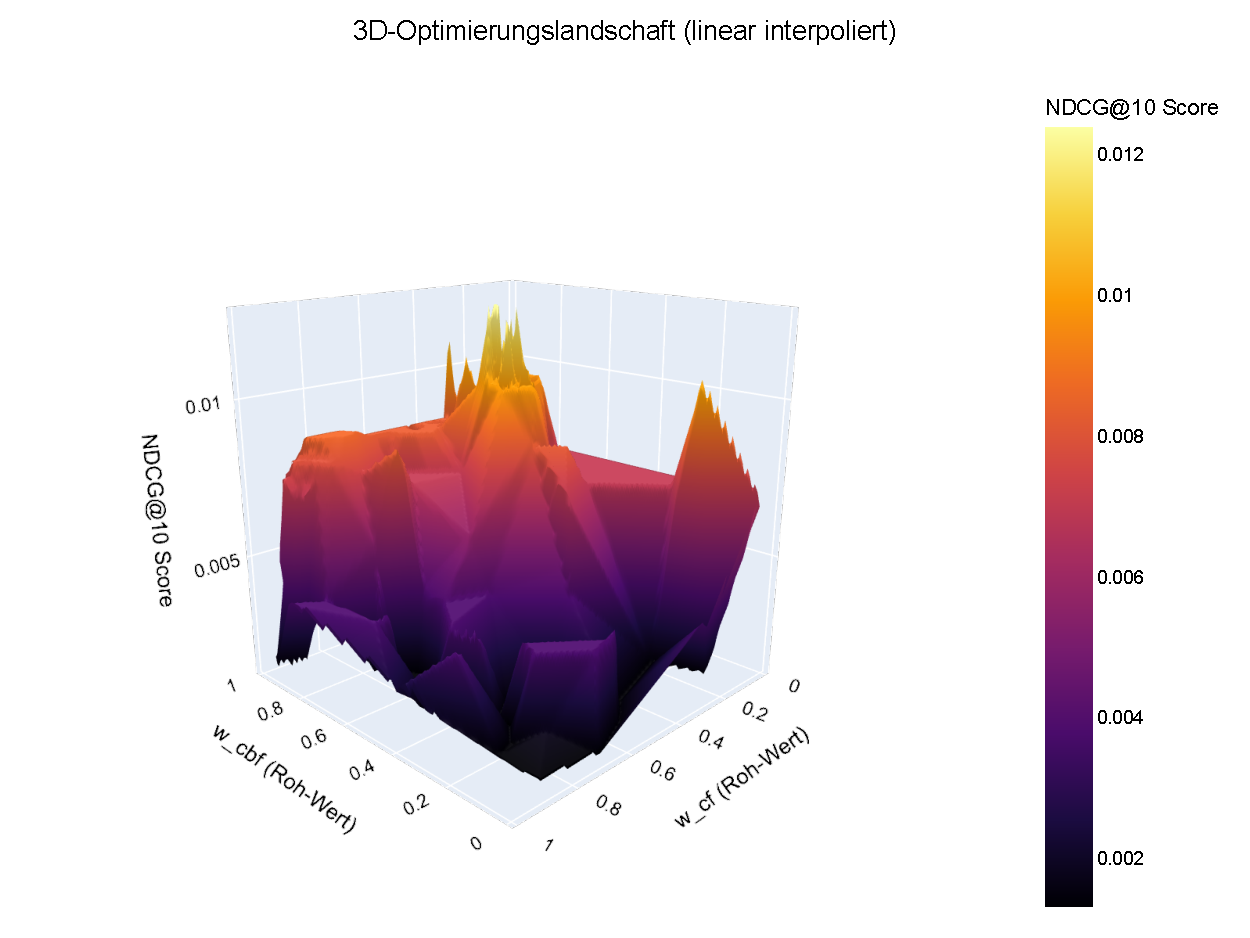
\includegraphics[width=0.9\textwidth]{content/figures/svg/hyperparameterraum.pdf}
    \caption{Visualisierung des zweidimensionalen Hyperparameterraums der Modellgewichtungen. Die Achsen repräsentieren die Gewichte für das CBF-Modell (\(w_{cbf}\)) und das CF-Modell (\(w_{cf}\)). Die Einfärbung der Punkte visualisiert den resultierenden NDCG@10-Wert für jede Konfiguration aus dem Optuna-Suchlauf.}
    \label{fig:hyperparameterraum}
\end{figure}

\subsection{Ergebnisse}
% % Tabellen: Precision@5, APS je α
% % Inhalt von: content/tables/vergleich_baselines.tex

\begin{table}[htbp]
    \centering
    \caption{Vergleich des optimierten Hybrid-Modells mit den Baseline-Modellen anhand der Metriken NDCG@10 und Hit Rate@10.}
    \label{tab:baseline_vergleich}
    \begin{tabular}{lrr}
        \toprule
        \textbf{Modell} & \textbf{NDCG@10} & \textbf{Hit Rate@10} \\
        \midrule
        Unser Hybrid-Modell (Final) & 1.25\% & 1.8\% \\
        Popularity-Baseline        & 0.23\% & 0.6\% \\
        Recency-Baseline           & 0.14\% & 0.4\% \\
        \bottomrule
    \end{tabular}
\end{table}
% % Visualisierungen: Liniendiagramme, ggf. UMAP-Spaces
% % content/tables/statistiken_testdaten.tex

\begin{table}[htbp]
    \centering
    \caption{Statistische Kennzahlen des Test- und Validierungsdatensatzes, basierend auf den Klick-Logs der letzten Januarwoche.}
    \label{tab:statistiken_test}
    \begin{tabular}{lr}
        \toprule
        \textbf{Metrik} & \textbf{Wert} \\
        \midrule
        Gesamte Artikelaufrufe & 3.627.024 \\
        Einzigartige user\_pseudo\_ids & 1.099.289 \\
        Einzigartige Artikel & 57.100 \\
        \bottomrule
    \end{tabular}
\end{table}
% % content/tables/statistiken_trainingsdaten.tex

\begin{table}[H]
    \centering
    \caption{Statistische Kennzahlen des Trainingsdatensatzes, basierend auf den Klick-Logs der ersten drei Januarwochen.}
    \label{tab:statistiken_training}
    \begin{tabular}{lr}
        \toprule
        \textbf{Metrik} & \textbf{Wert} \\
        \midrule
        Gesamte Interaktionen (Klicks) & 11.412.116 \\
        Einzigartige user\_pseudo\_ids & 2.294.733 \\
        Einzigartige Artikel & 104.462 \\
        \bottomrule
    \end{tabular}
\end{table}
% % content/figures/plot_nutzerverteilung_test.tex

\begin{figure}[H]
    \centering
    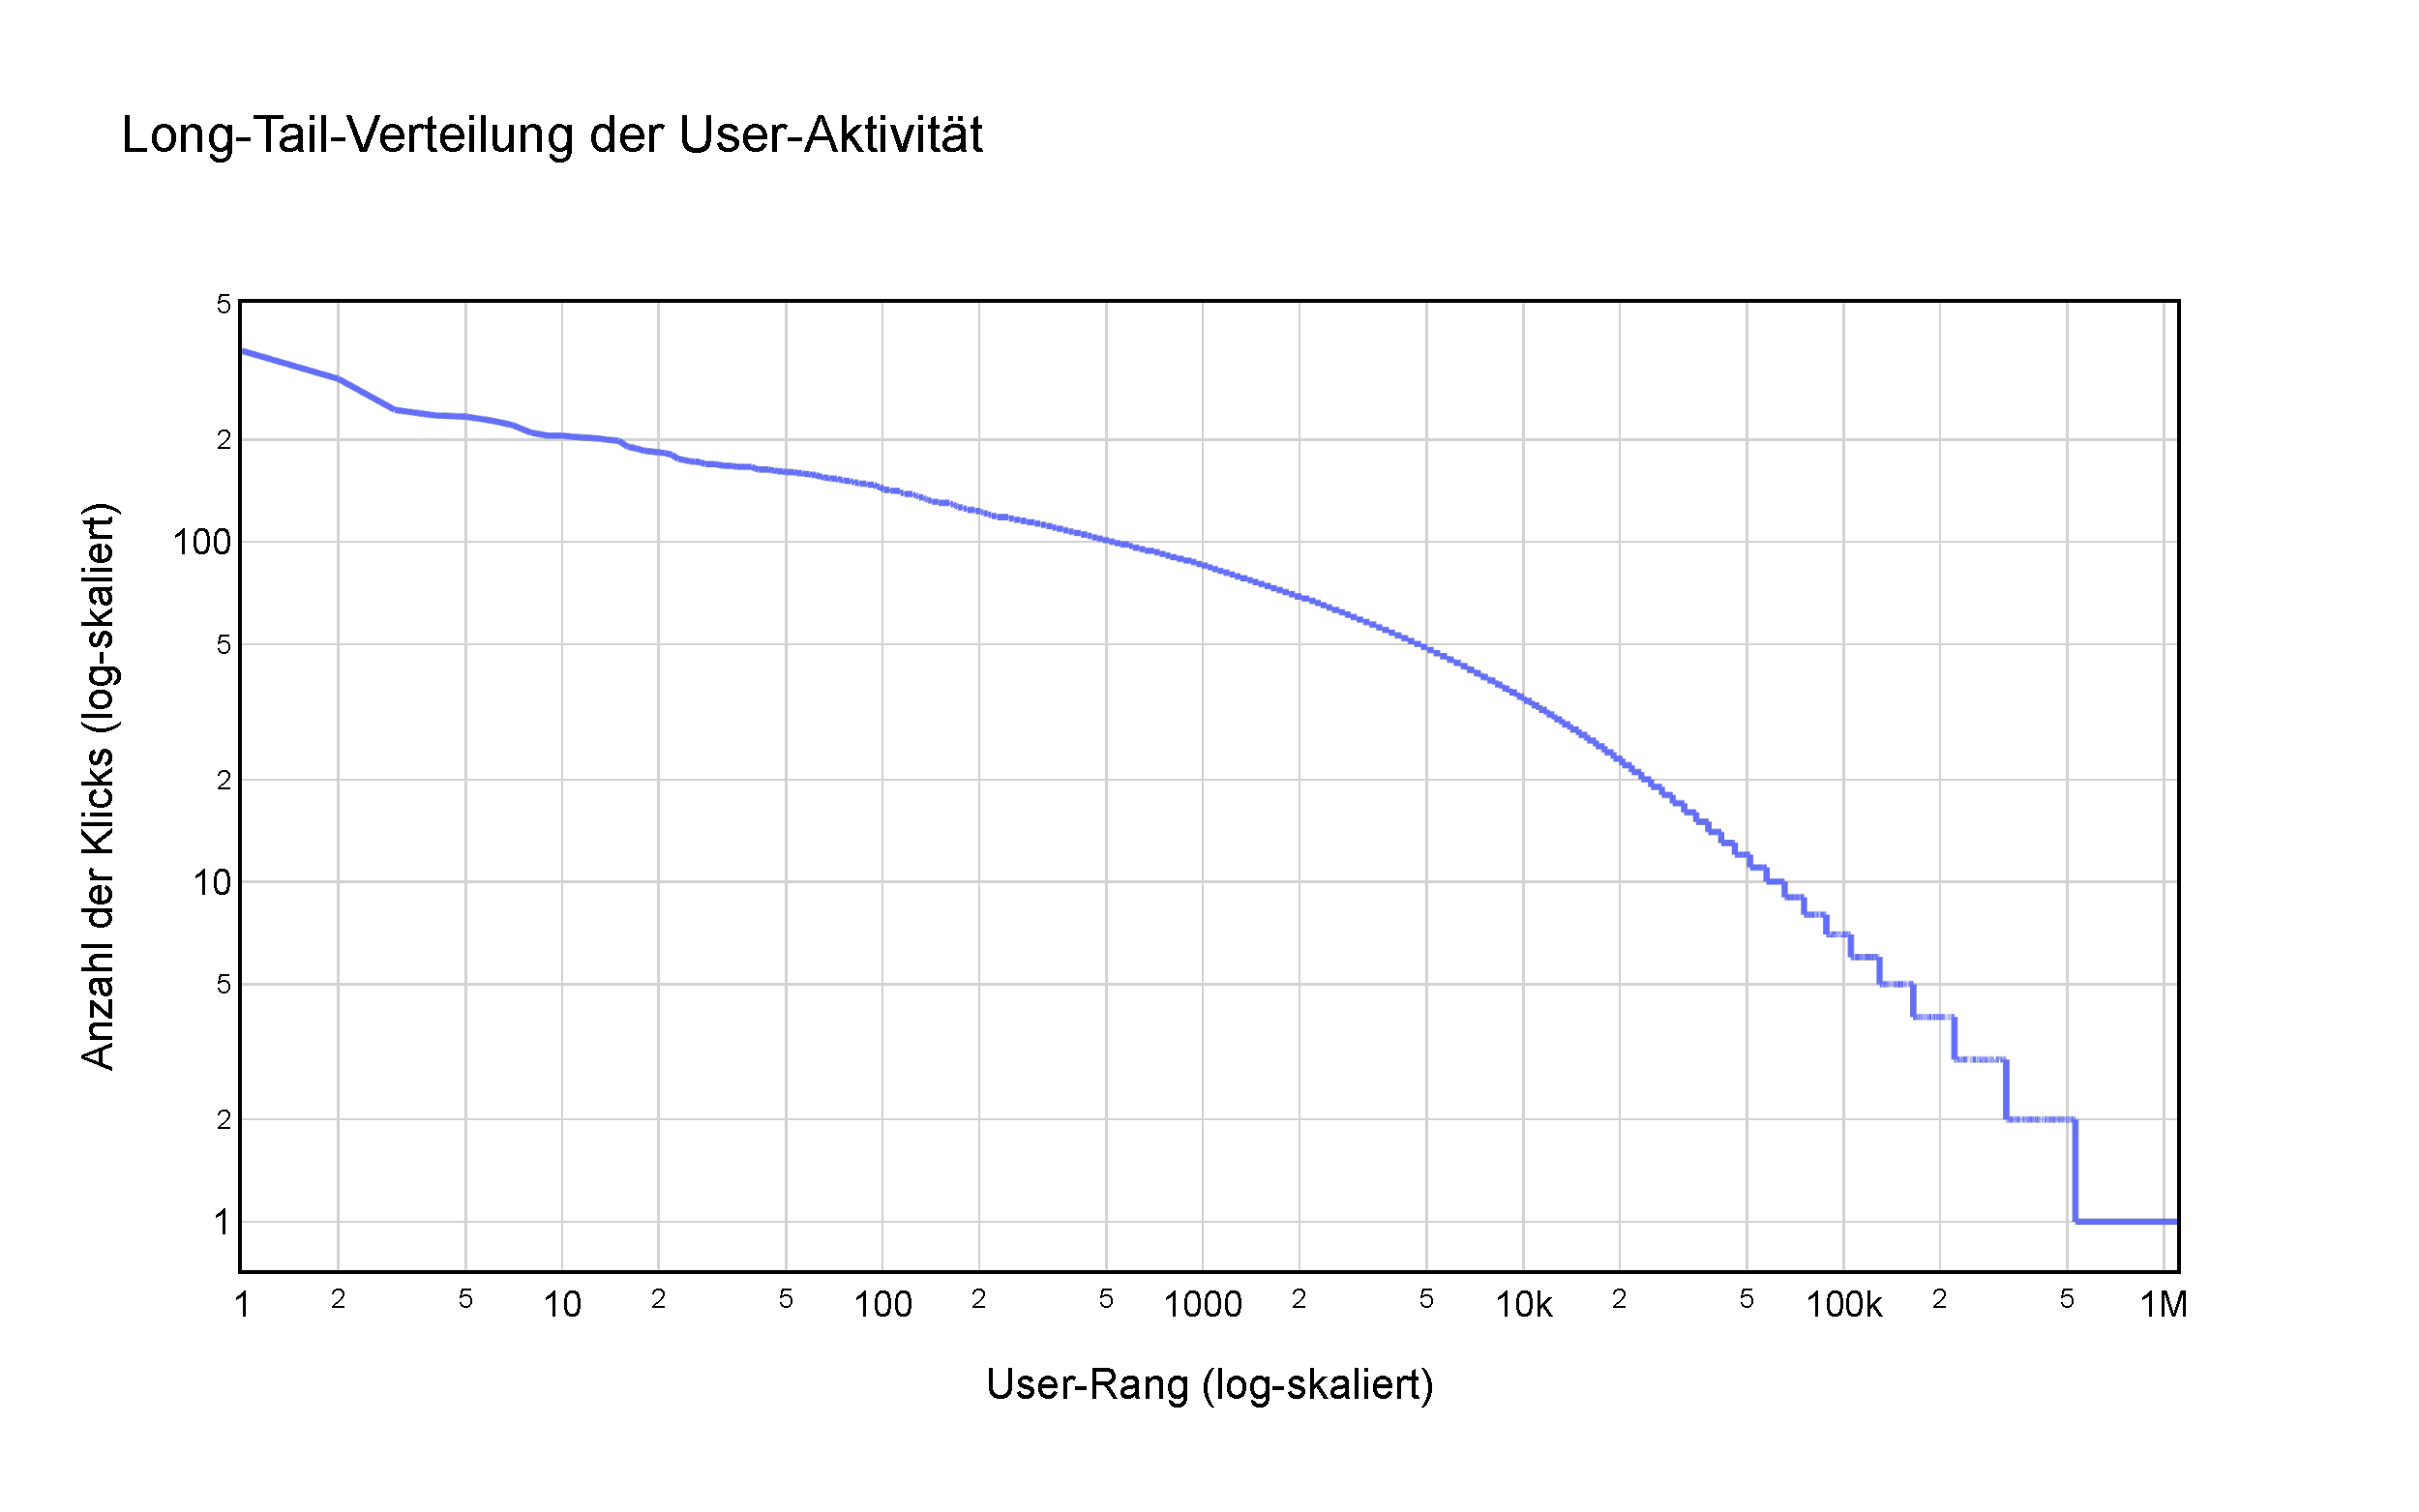
\includegraphics[width=0.9\textwidth]{content/figures/svg/nutzer_verteilung_test.pdf}
    \caption{Verteilung der Nutzeraktivität im Testdatensatz. Die Verteilung ist analog zum Trainingsdatensatz und zeigt ebenfalls eine ausgeprägte Long-Tail-Struktur, was die Repräsentativität des Test-Splits unterstreicht.}
    \label{fig:nutzerverteilung_test}
\end{figure}
% % content/figures/plot_nutzerverteilung_train.tex

\begin{figure}[H]
    \centering
    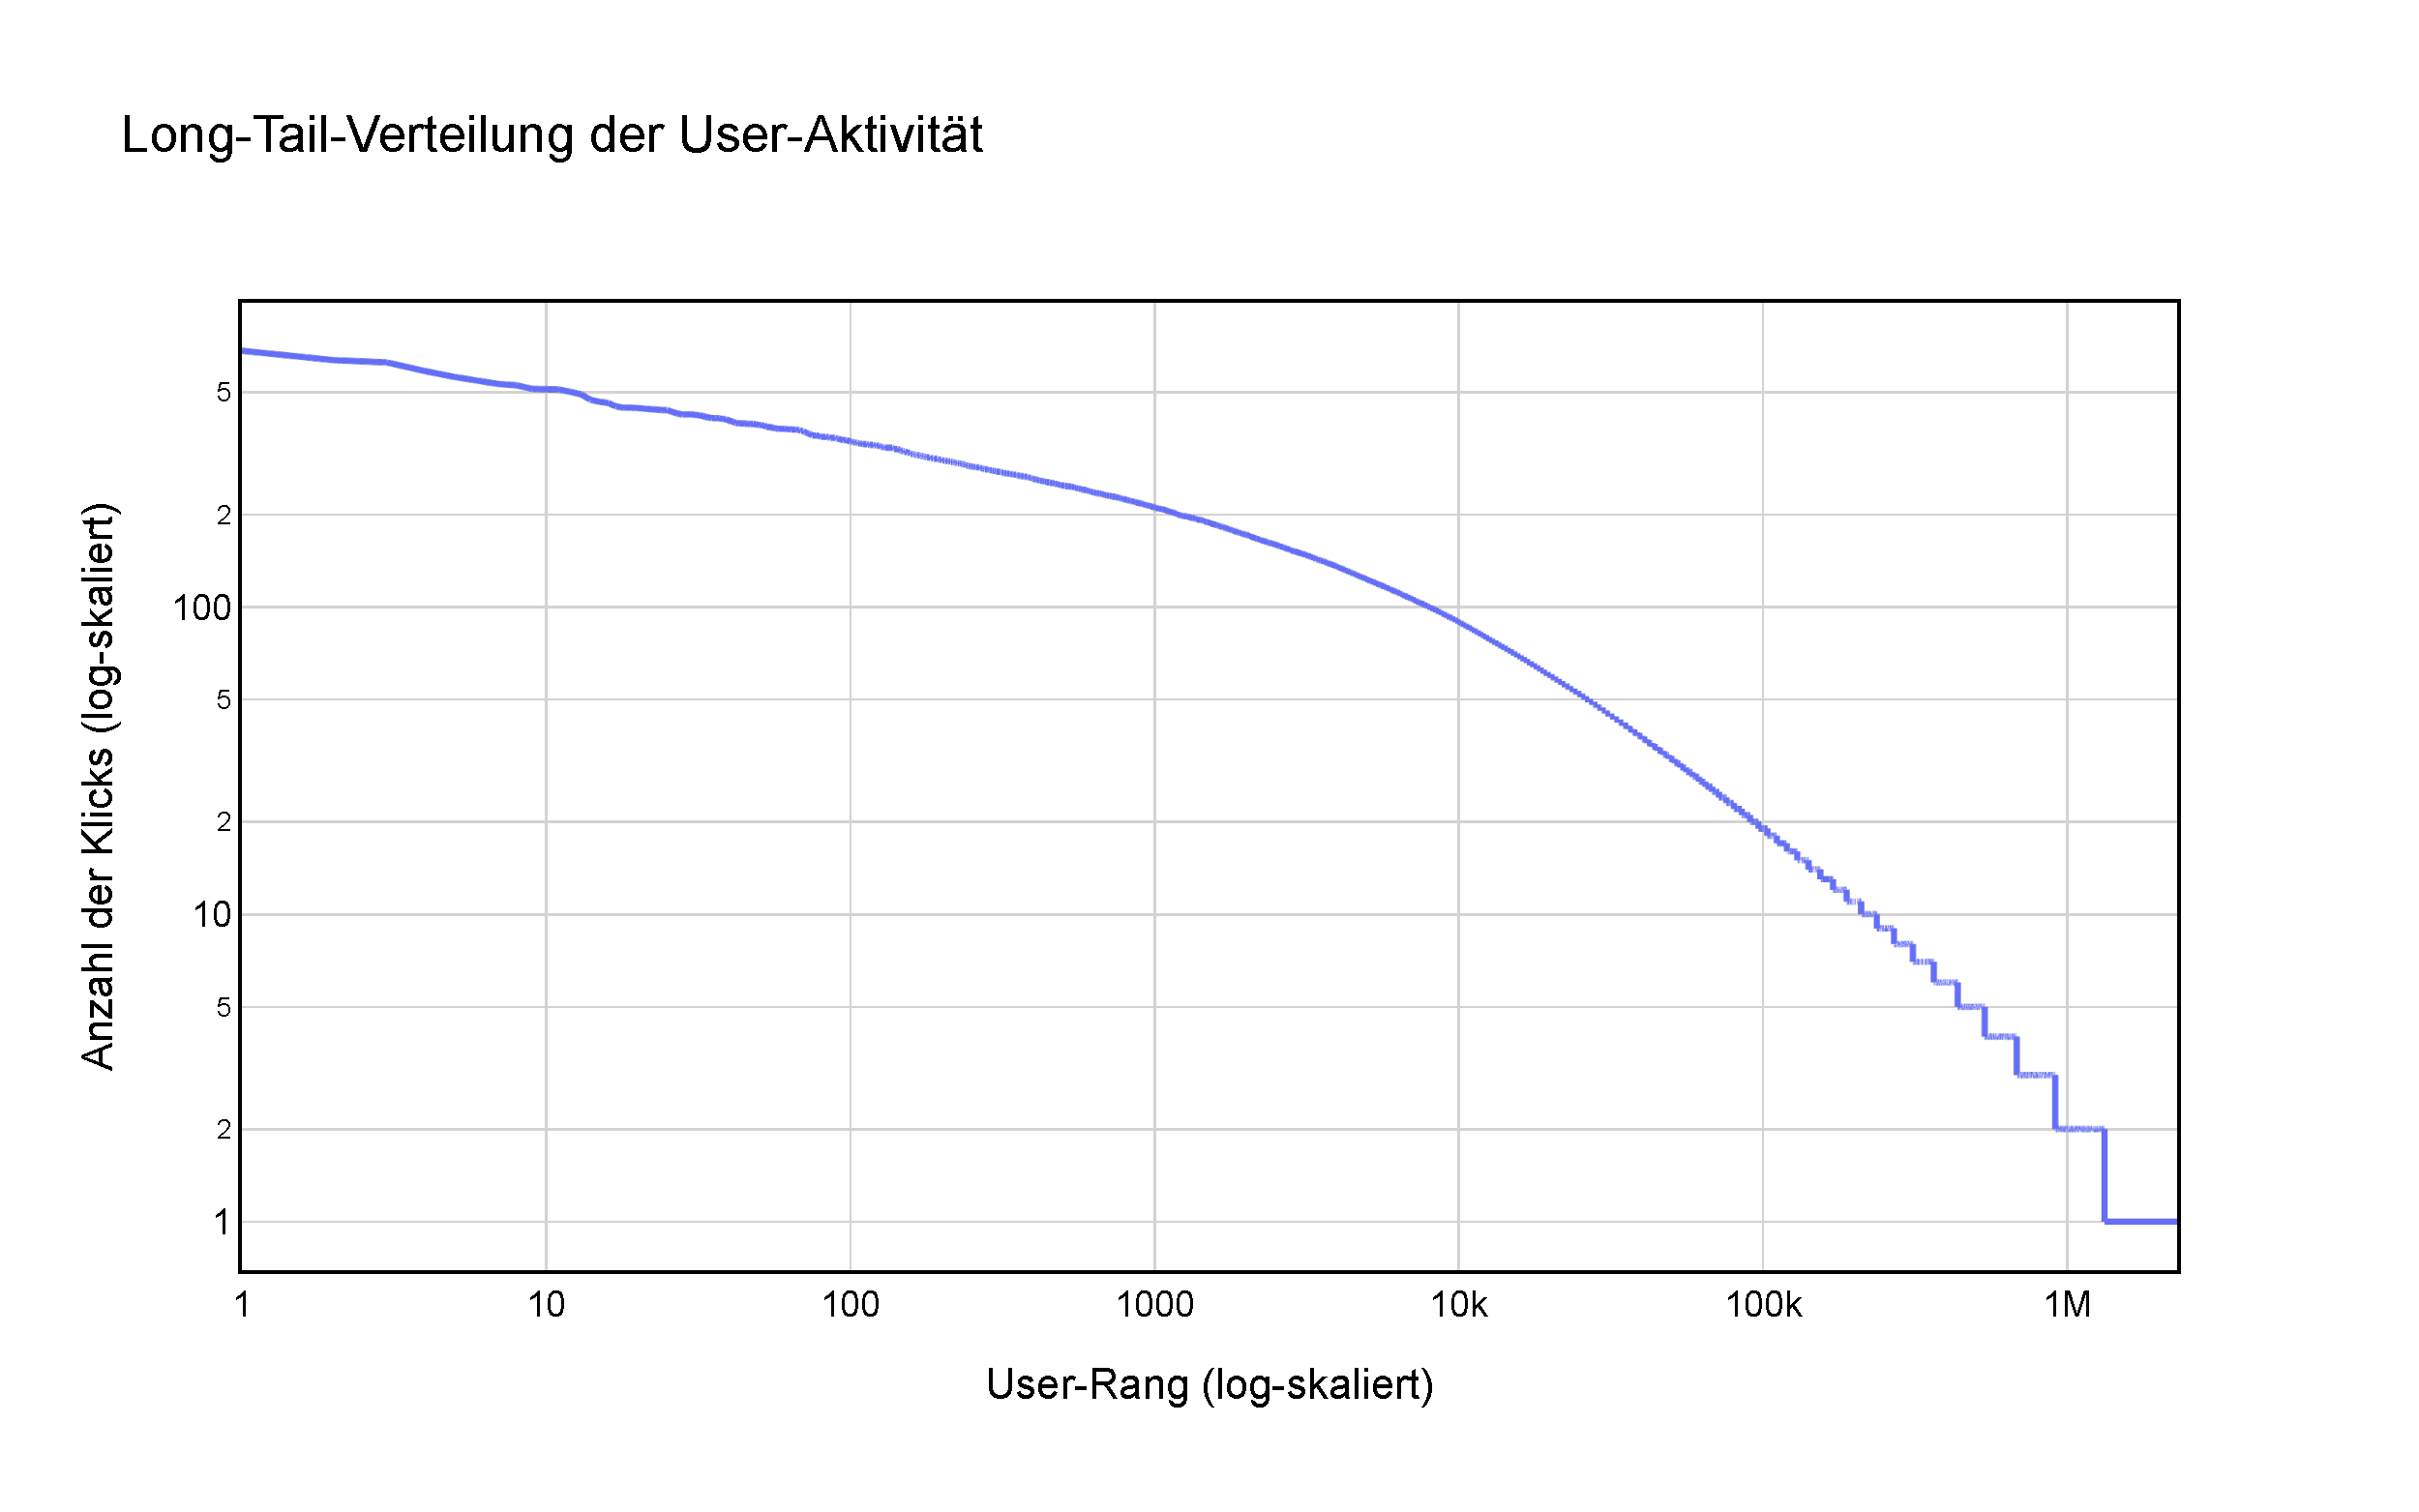
\includegraphics[width=0.9\textwidth]{content/figures/svg/nutzer_verteilung_train.pdf}
    \caption{Verteilung der Nutzeraktivität im Trainingsdatensatz. Die Darstellung verdeutlicht die typische Long-Tail-Verteilung: Eine große Anzahl von Nutzern interagiert nur selten mit Artikeln, während eine kleine Gruppe von "Power-Nutzern" für einen Großteil der Klicks verantwortlich ist.}
    \label{fig:nutzerverteilung_train}
\end{figure}
% % content/figures/plot_artikelverteilung_test.tex

\begin{figure}[htbp]
    \centering
    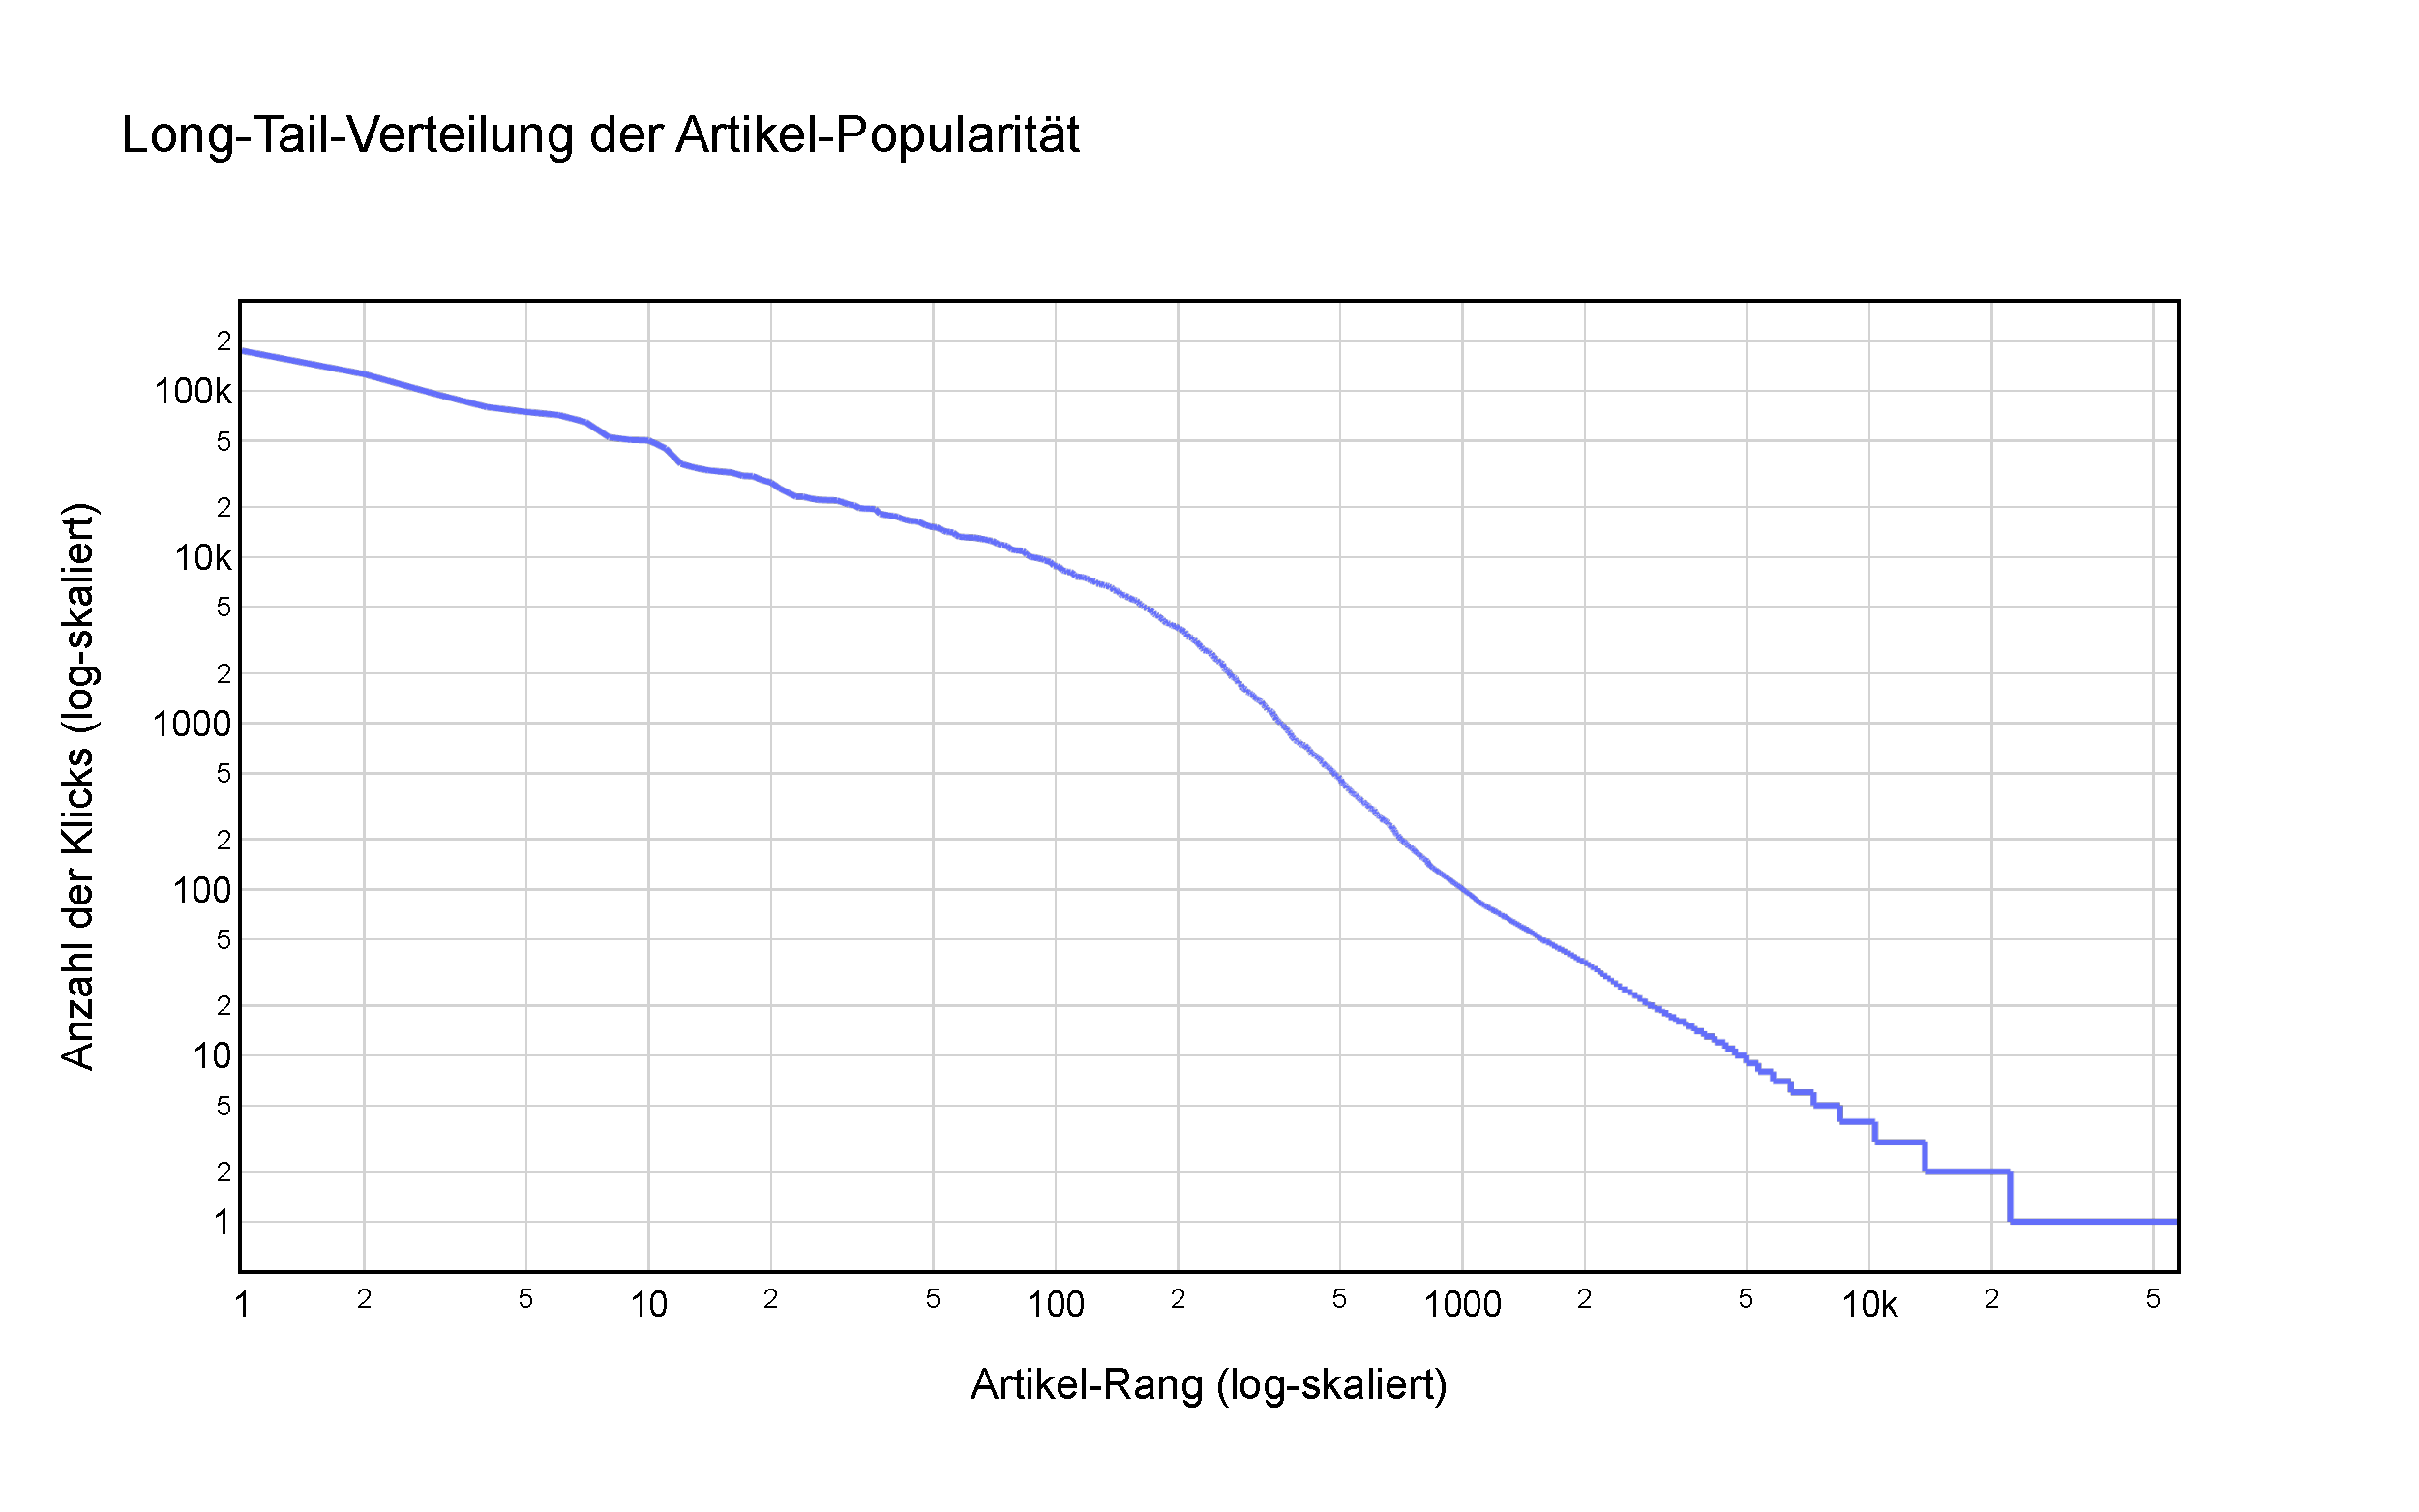
\includegraphics[width=0.9\textwidth]{content/figures/svg/artikel_verteilung_test.pdf}
    \caption{Popularitätsverteilung der Artikel im Testdatensatz. Die charakteristische Long-Tail-Verteilung bleibt auch in der letzten Januarwoche bestehen, was auf eine stabile Grundstruktur des Nutzerinteresses hindeutet.}
    \label{fig:artikelverteilung_test}
\end{figure}
% % content/figures/plot_artikelverteilung_train.tex

\begin{figure}[H]
    \centering
    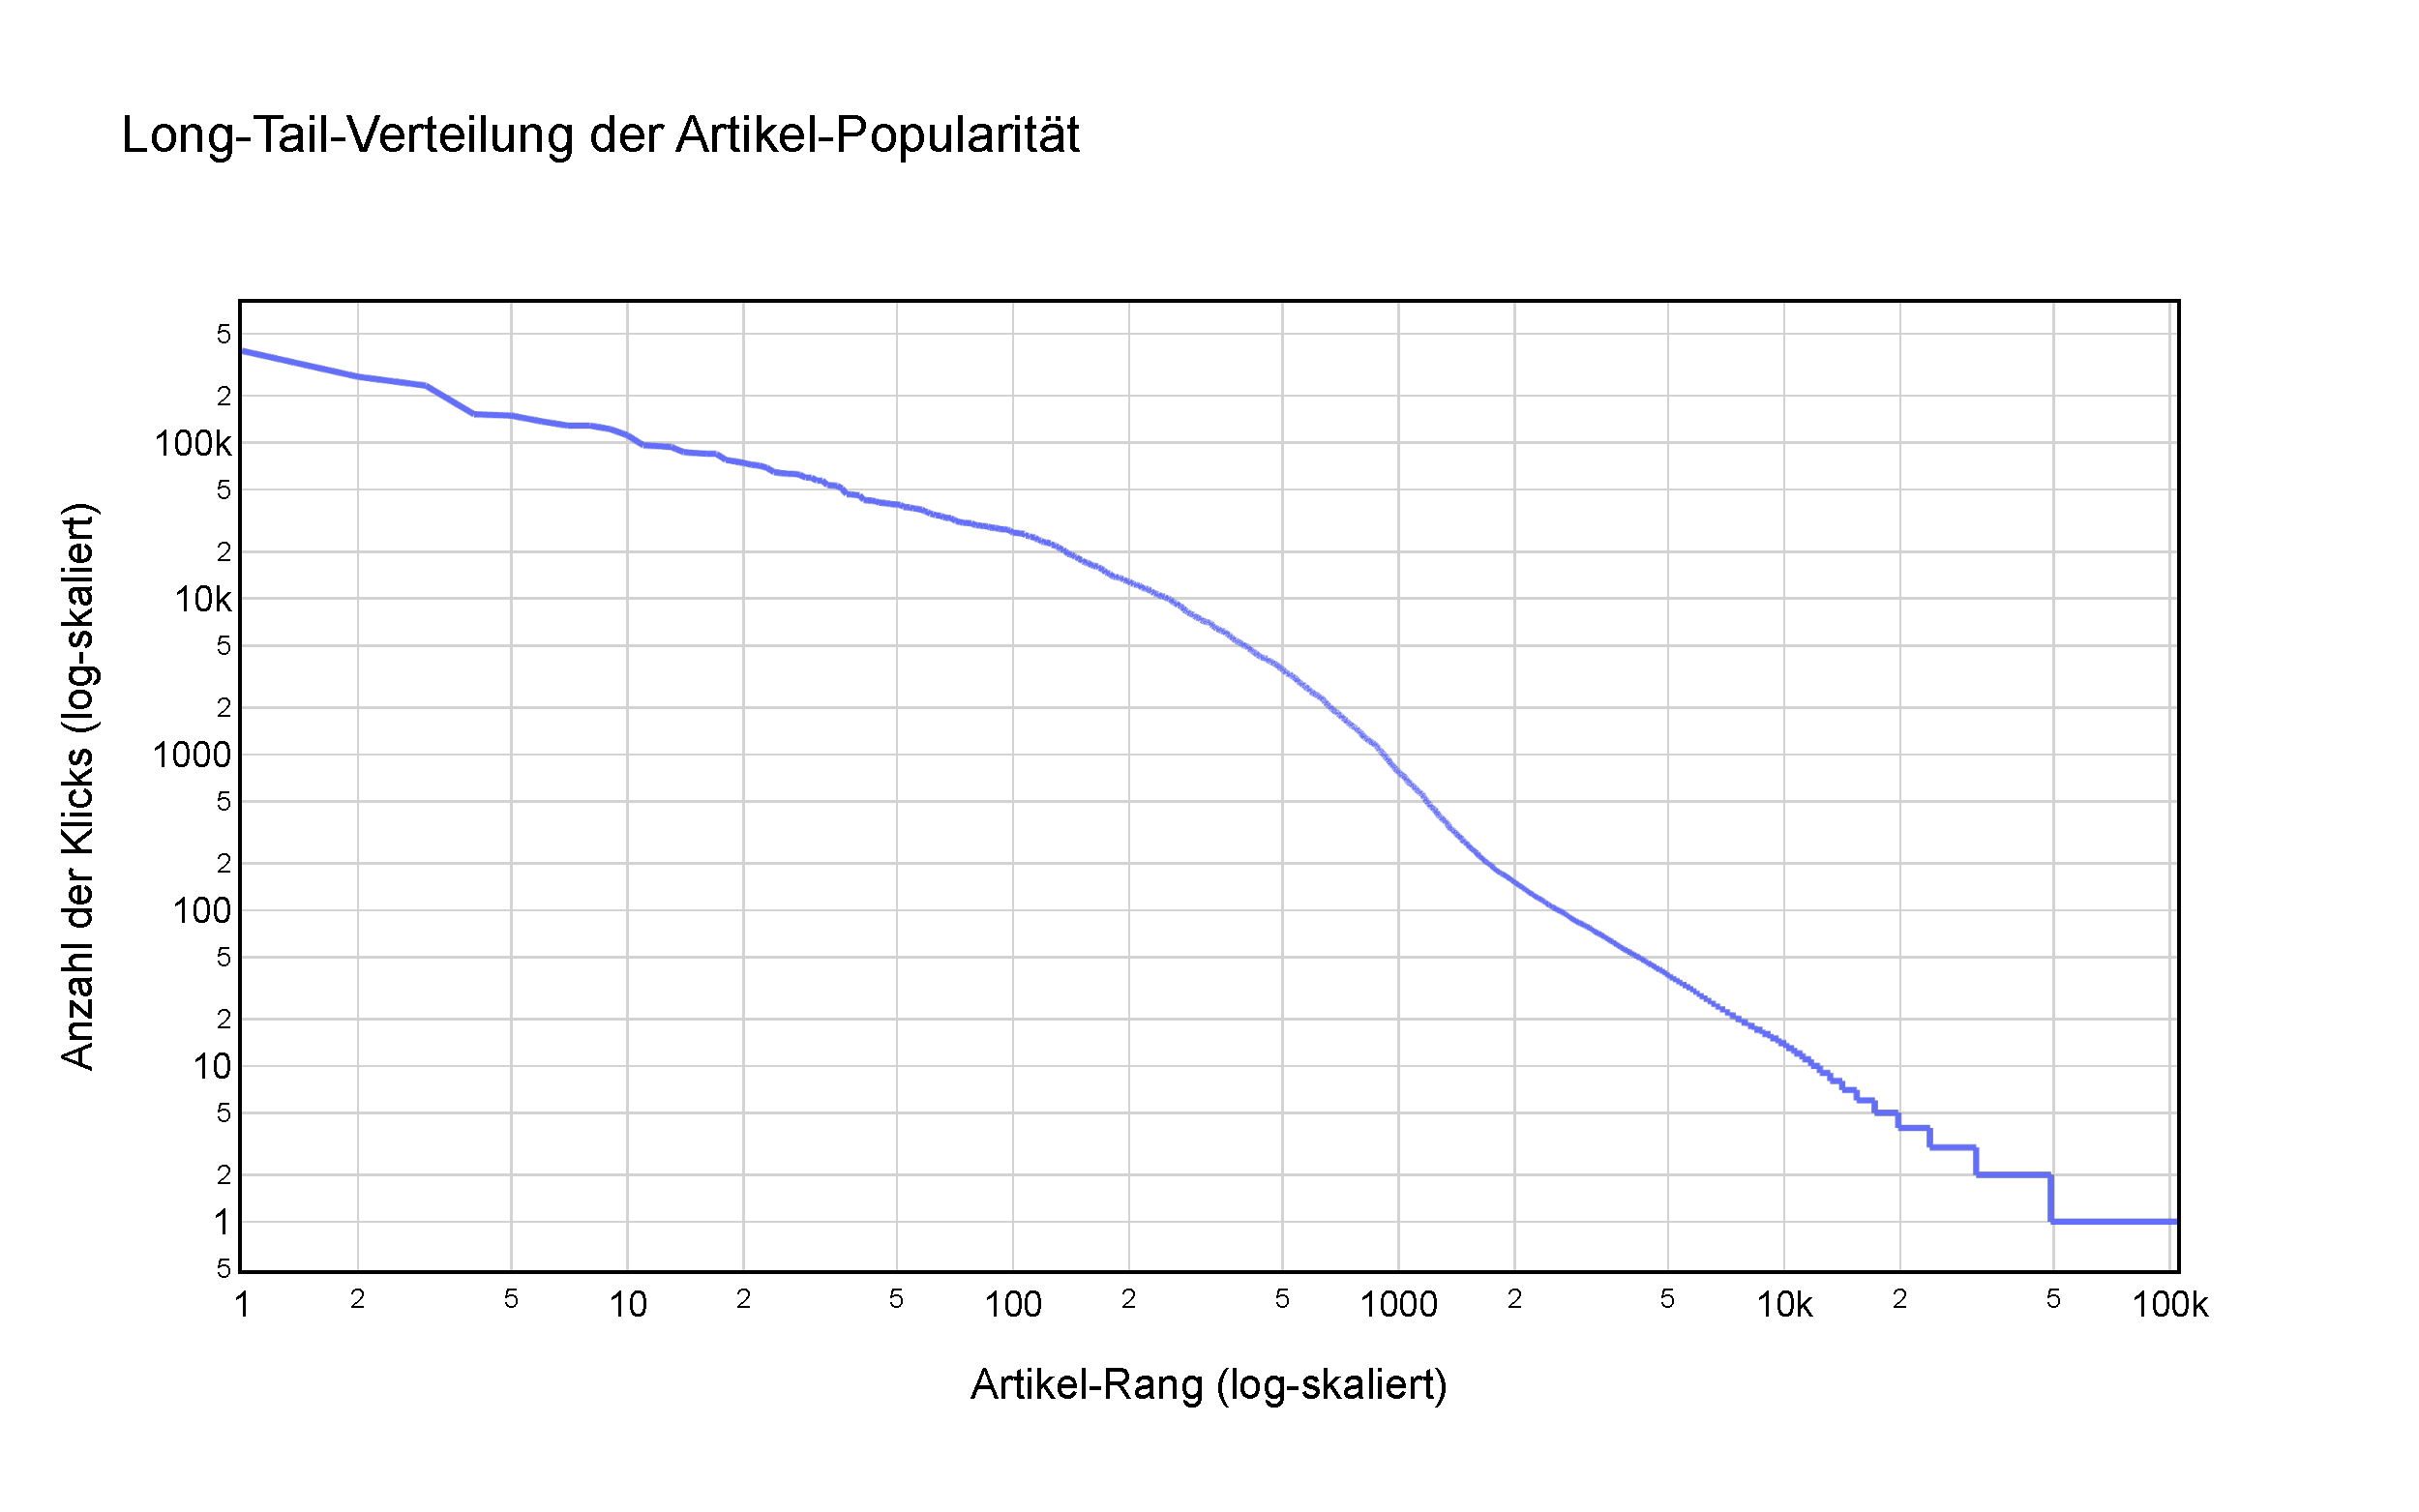
\includegraphics[width=0.9\textwidth]{content/figures/svg/artikel_verteilung_train.pdf}
    \caption{Popularitätsverteilung der Artikel im Trainingsdatensatz. Die Grafik zeigt, dass eine geringe Anzahl von Artikeln einen Großteil der Klicks auf sich vereint, während die Mehrheit der Artikel nur wenige Interaktionen erhält (Long-Tail).}
    \label{fig:artikelverteilung_train}
\end{figure}
% \subsection{Interpretation und Analyse}
% % Hybridisierung wirkungsvoll?
% % Trade-offs und Nutzenklärung
% % Ablationsidee: z. B. Ausschalten von CBF-/CF-Signal
% % content/figures/plot_2d_performance.tex

\begin{figure}[H]
    \centering
    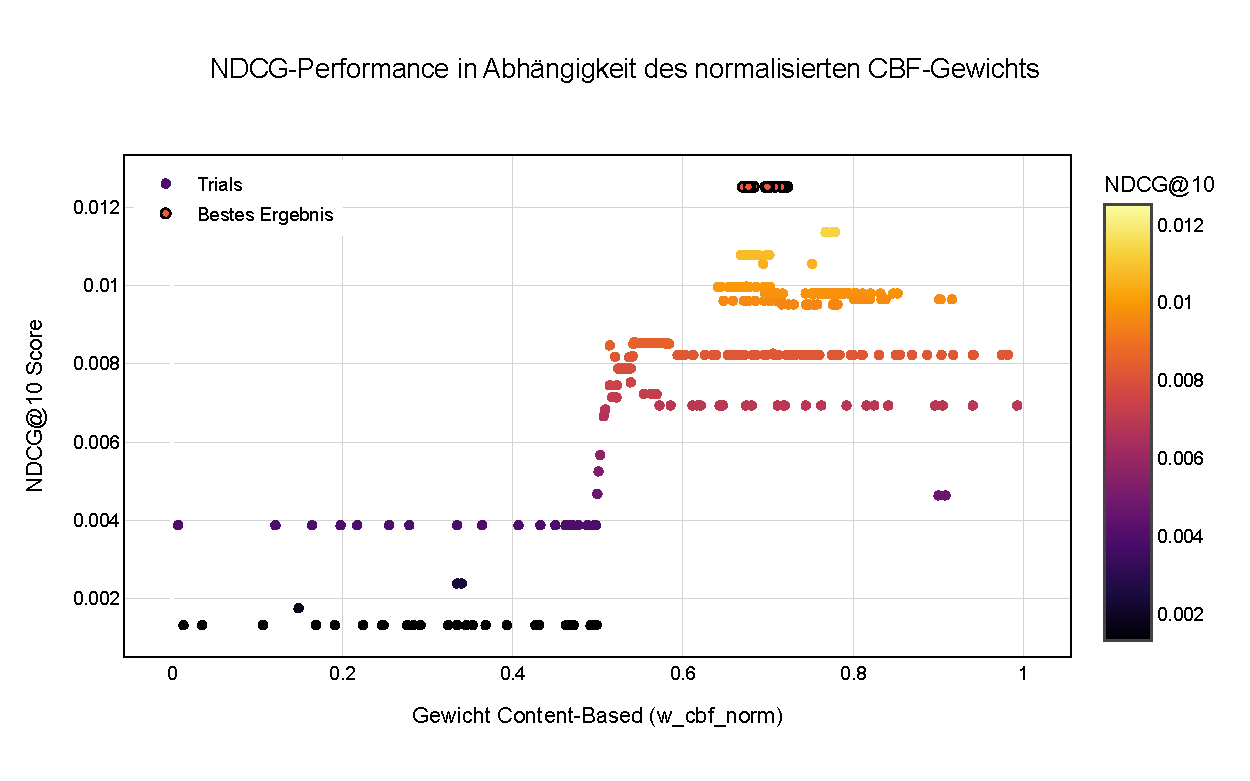
\includegraphics[width=0.9\textwidth]{content/figures/svg/2d_performance.pdf}
    \caption{2D-Darstellung des Hyperparameterraums. Die Achsen zeigen die Gewichtungen für das CBF- (\(w_{cbf}\)) und CF-Modell (\(w_{cf}\)). Die Farbe der Punkte indiziert den erreichten NDCG@10-Score. Der optimale Punkt ist markiert.}
    \label{fig:2d_performance}
\end{figure}
% % content/figures/plot_3d_scatter.tex

\begin{figure}[htbp]
    \centering
    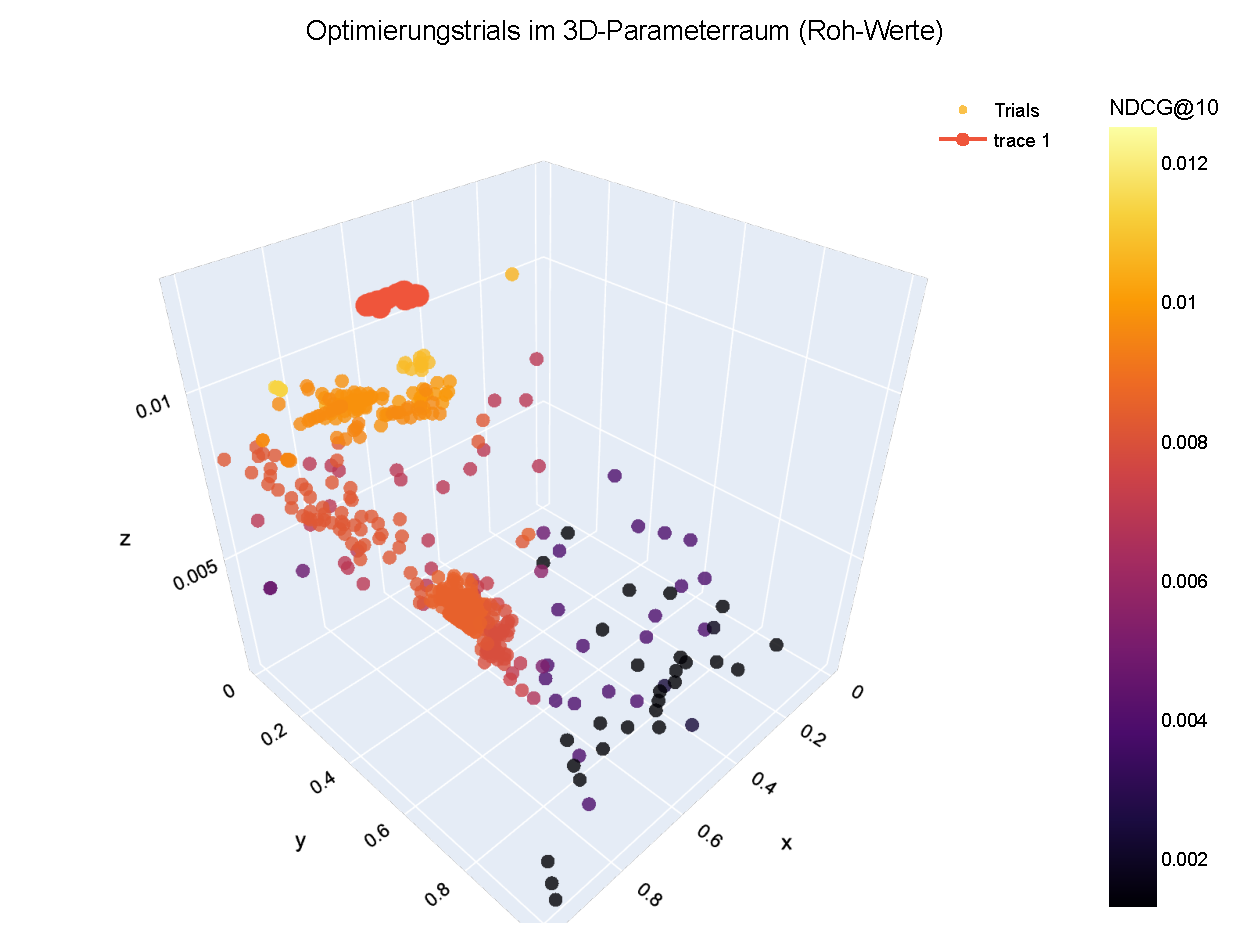
\includegraphics[width=0.8\textwidth]{content/figures/svg/3d_scatter_plot.pdf}
    \caption{Interaktives 3D-Streudiagramm der Optuna-Trials zur Visualisierung der Parameterabhängigkeiten. (Hinweis: Die Darstellung in der PDF-Version der Arbeit ist eine statische Ansicht).}
    \label{fig:3d_scatter}
\end{figure}
% % content/figures/plot_kontour.tex

\begin{figure}[htbp]
    \centering
    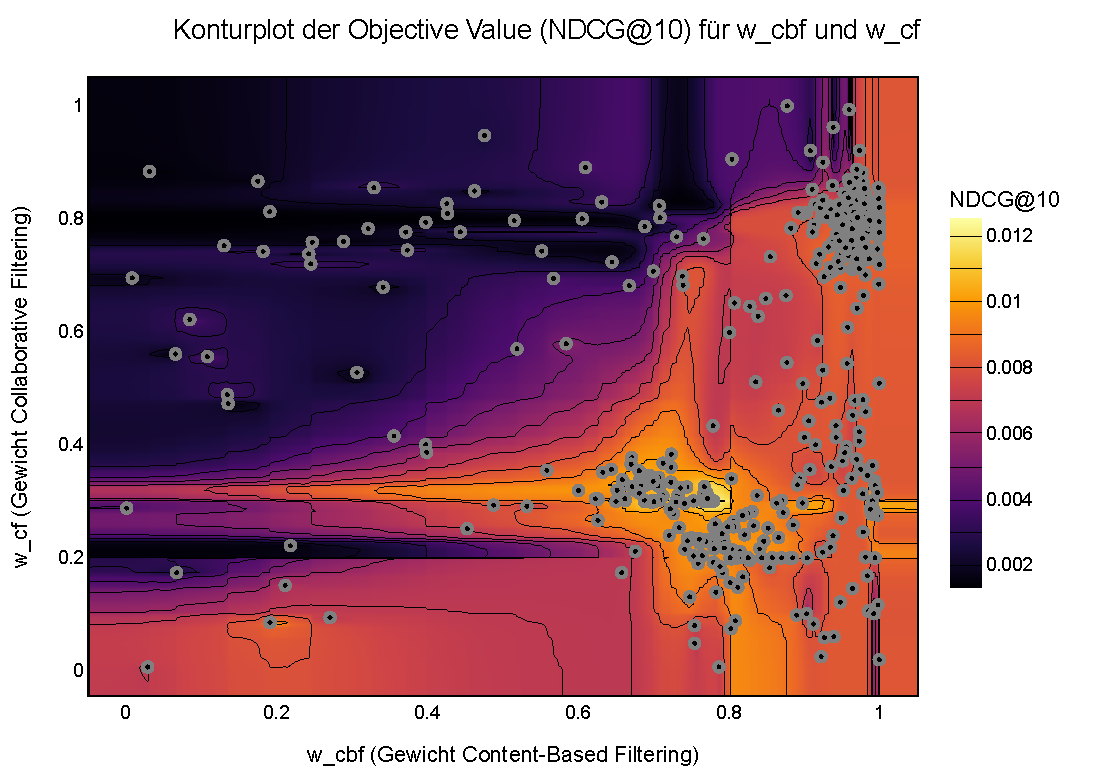
\includegraphics[width=0.9\textwidth]{content/figures/svg/kontourplot.pdf}
    \caption{Konturplot zur Darstellung der NDCG@10-Verteilung im zweidimensionalen Parameterraum der Modellgewichtungen. Die Isolinien verbinden Bereiche mit ähnlicher Performance.}
    \label{fig:kontourplot}
\end{figure}
% % content/figures/plot_optimierungsverlauf.tex

\begin{figure}[htbp]
    \centering
    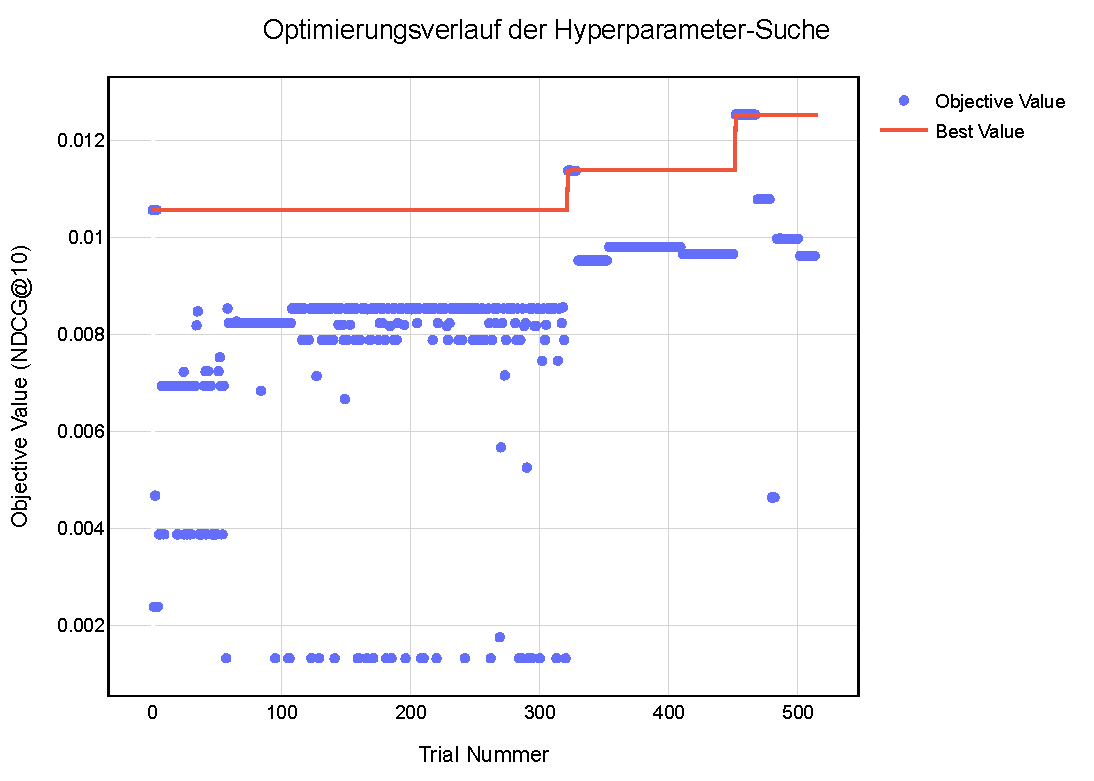
\includegraphics[width=0.9\textwidth]{content/figures/svg/optimierungsverlauf.pdf}
    \caption{Visualisierung des Optimierungsverlaufs der 515 Optuna-Trials. Jeder Punkt stellt die NDCG@10-Metrik (Y-Achse) für einen bestimmten Trial (X-Achse) dar. Der Verlauf zeigt die Konvergenz des Optimierers gegen bessere Werte.}
    \label{fig:optimierungsverlauf}
\end{figure}
% % content/figures/plot_hyperparameterraum.tex

\begin{figure}[H]
    \centering
    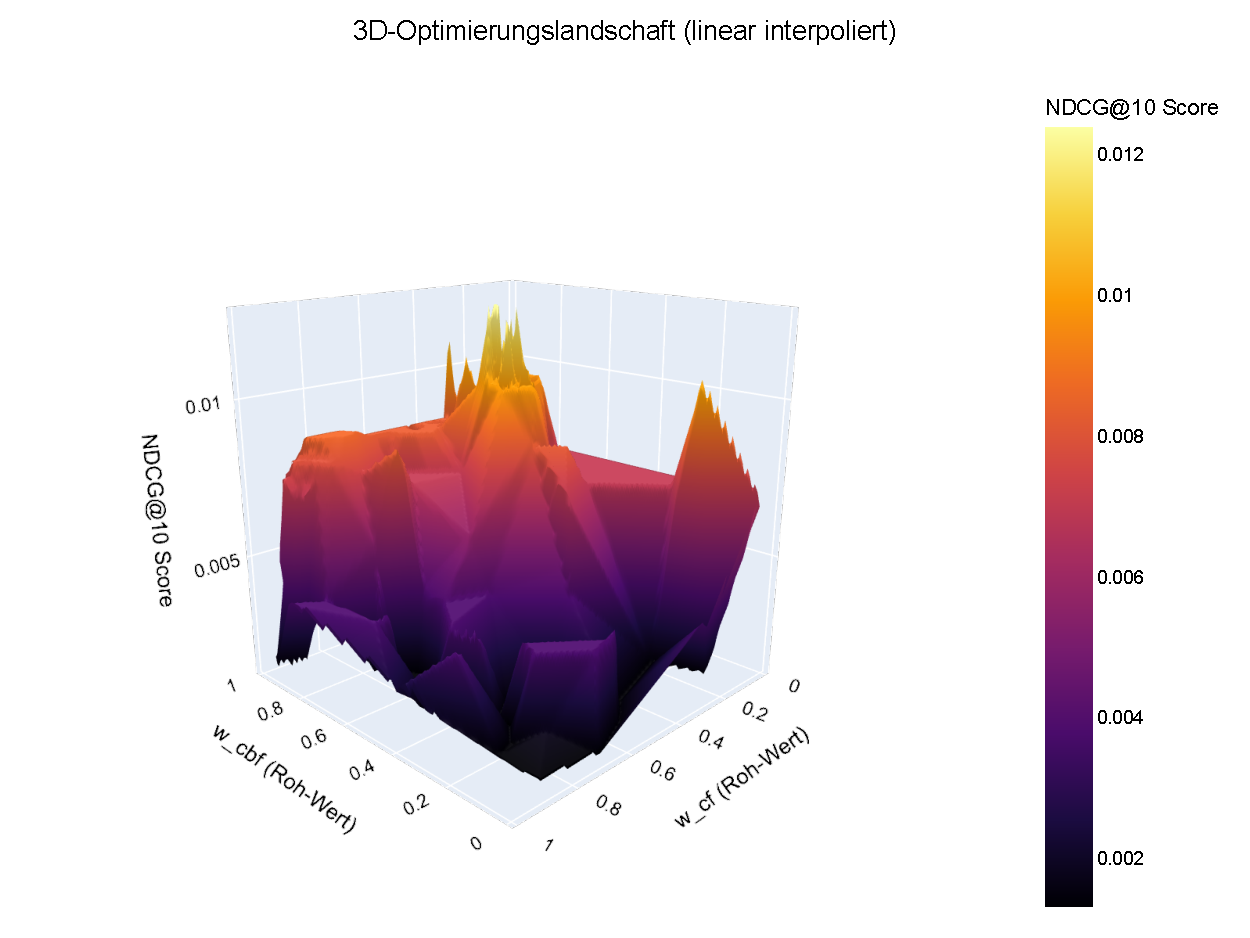
\includegraphics[width=0.9\textwidth]{content/figures/svg/hyperparameterraum.pdf}
    \caption{Visualisierung des zweidimensionalen Hyperparameterraums der Modellgewichtungen. Die Achsen repräsentieren die Gewichte für das CBF-Modell (\(w_{cbf}\)) und das CF-Modell (\(w_{cf}\)). Die Einfärbung der Punkte visualisiert den resultierenden NDCG@10-Wert für jede Konfiguration aus dem Optuna-Suchlauf.}
    \label{fig:hyperparameterraum}
\end{figure}